\chapter{Implementacija i korisničko sučelje}
		
		
		\section{Korištene tehnologije i alati}
		
			\textbf{\textit{dio 2. revizije}}
			
			 \textit{Detaljno navesti sve tehnologije i alate koji su primijenjeni pri izradi dokumentacije i aplikacije. Ukratko ih opisati, te navesti njihovo značenje i mjesto primjene. Za svaki navedeni alat i tehnologiju je potrebno \textbf{navesti internet poveznicu} gdje se mogu preuzeti ili više saznati o njima}.
			
			
			\eject 
		
	
		\section{Ispitivanje programskog rješenja}
			
			\textbf{\textit{dio 2. revizije}}\\
			
			 \textit{U ovom poglavlju je potrebno opisati provedbu ispitivanja implementiranih funkcionalnosti na razini komponenti i na razini cijelog sustava s prikazom odabranih ispitnih slučajeva. Studenti trebaju ispitati temeljnu funkcionalnost i rubne uvjete..}
	
			
			\subsection{Ispitivanje komponenti}
			\textit{Potrebno je provesti ispitivanje jedinica (engl. unit testing) nad razredima koji implementiraju temeljne funkcionalnosti. Razraditi \textbf{minimalno 6 ispitnih slučajeva} u kojima će se ispitati redovni slučajevi, rubni uvjeti te izazivanje pogreške (engl. exception throwing). Poželjno je stvoriti i ispitni slučaj koji koristi funkcionalnosti koje nisu implementirane. Potrebno je priložiti izvorni kôd svih ispitnih slučajeva te prikaz rezultata izvođenja ispita u razvojnom okruženju (prolaz/pad ispita). }
			
			
			
			\subsection{Ispitivanje sustava}
			
			 Ispitivanje sustava obavili smo koristeći radni okvir Selenium. Ispitivanje se radilo po obrascima uporabe kako bi se provjerile osnovne funkcionalnosti sustava, ali i nasumičnim kretanjem po aplikaciji kako bi pronašli eventualne greške. Aplikacija prolazi svai ispitni slučaj koji smo testirali jer je testiranje napravljeno nakon dodavanja svih funkcionalnosti koje sustav treba imati.
			 
			 \text{}
			 
			 
		 	\textbf{Ispitni slučaj 1: Prijava korisnika u sustav} 
		 	
		 	\textbf{Ulaz}
		 	
		 	\begin{enumerate}
		 		
		 		\item Otvaranje početne stranice u web pregledniku.
		 		\item Upisivanje korisničkog imena i lozinke.
		 	\end{enumerate}
	 	
	 		\textbf{Očekivani rezultat}
	 		
	 		\begin{enumerate}
	 			\item Prikazuje se početna stranica web aplikacije s korisnikovim podacima.
	 		\end{enumerate}
			
			\textbf{Rezultat}: Očekivani rezultat je zadovoljen i nakon unosa korisničkog imena i lozinke, korisnik je prijavljen u sustav. Aplikacija je prošla test.
			
			\begin{figure}[H]
				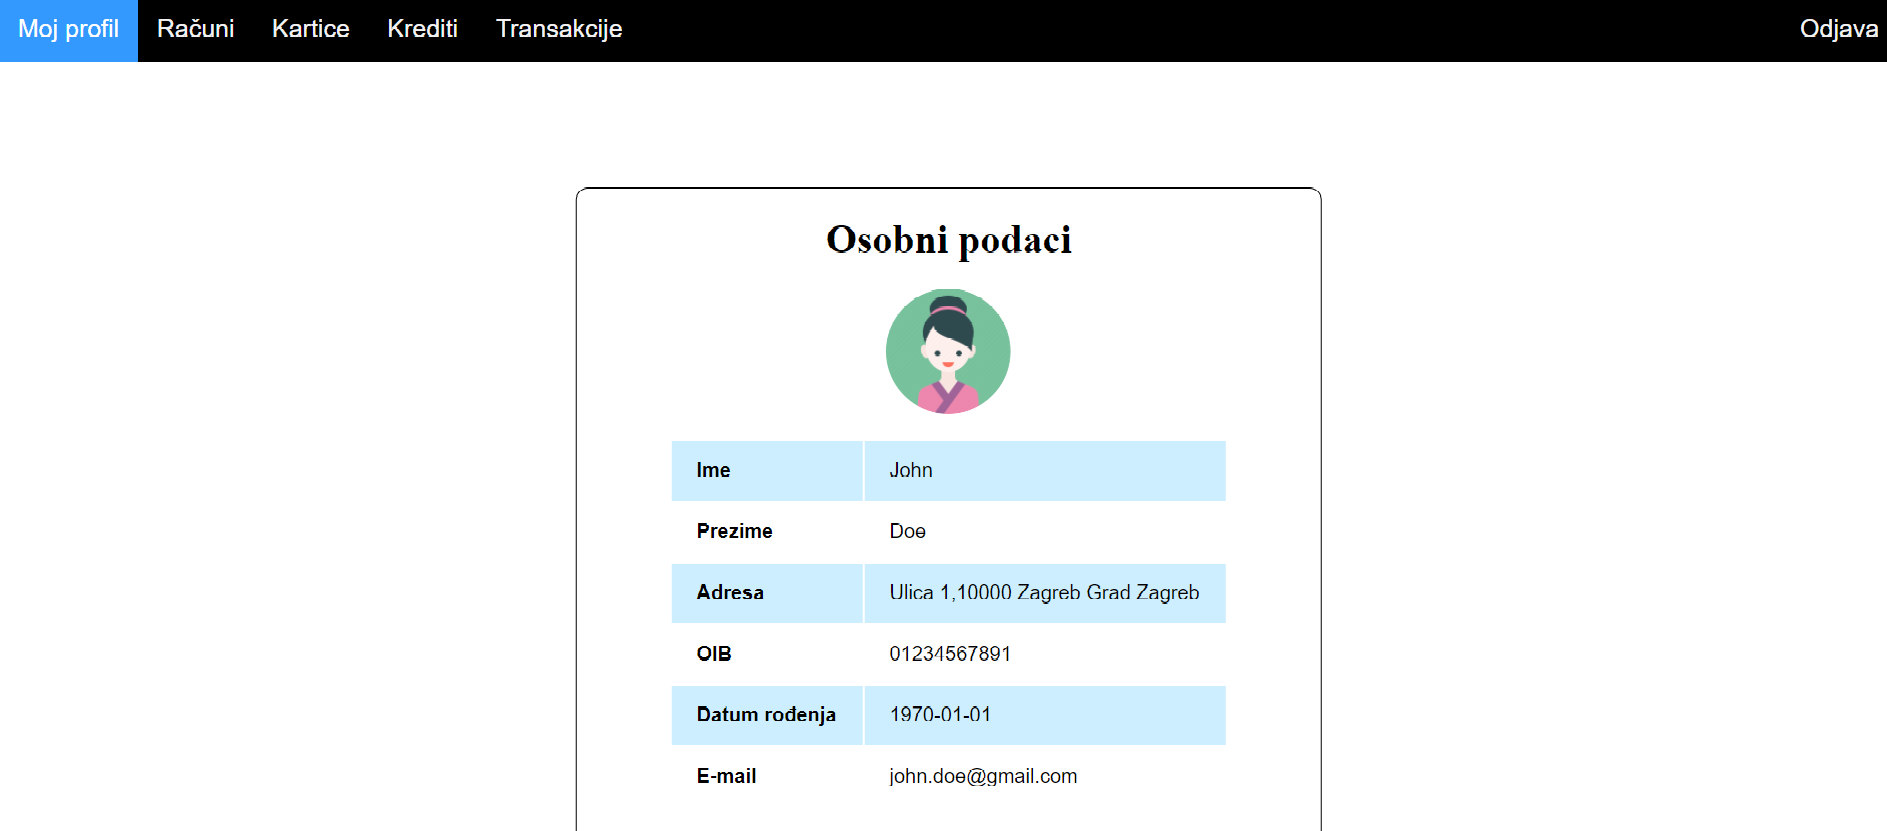
\includegraphics[scale=0.4]{slike/prijava.PNG}
				\centering
				\caption{Prijava u sustav}
				\label{fig:prijava}
			\end{figure}
		
		\textbf{Ispitni slučaj 2: Izrada nove kartice} 
		
		\textbf{Ulaz}
		
		\begin{enumerate}
			
			\item Otvaranje početne stranice u web pregledniku.
			\item Upisivanje korisničkog imena i lozinke klijenta.
			\item Odabir nove kartice koju korisnik želi napraviti.
			\item Prijava službenika u sustav.
			\item Odabir novih kartičnih zahtjeva.
			\item Službenik popunjava detalje o novoj kartici i odobrava zahtjev.
		\end{enumerate}
		
		\textbf{Očekivani rezultat}
		
		\begin{enumerate}
			\item Klijentu se u sustavu prikazuje novonastala kartica ukoliko je službenik odobrio zahtjev za izradom nove kartice.
			\item Klijent ima uvid o detaljima nove kartice.
		\end{enumerate}
		
		\textbf{Rezultat}: Očekivani rezultat je zadovoljen i nakon prijave u sustav, klijentu se pritiskom na gumb "Kartice" prikazuju sve kartice koje posjeduje. Aplikacija je prošla test.
		
		\begin{figure}[H]
			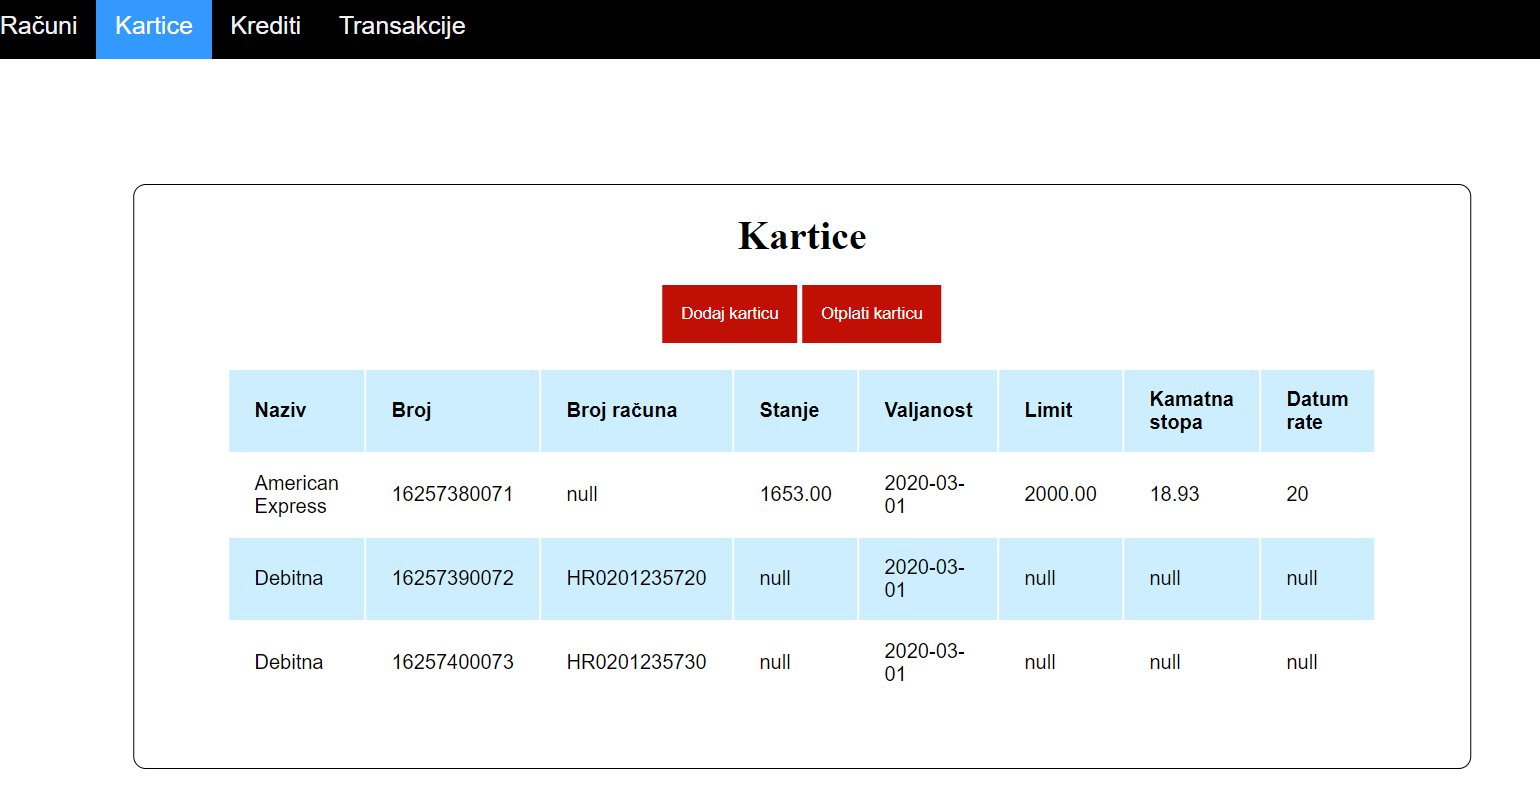
\includegraphics[scale=0.5]{slike/karticeprije.PNG}
			\centering
			\caption{Prikaz kartica prije odobravanja zahtjeva za novom karticom}
			\label{fig:prije}
		\end{figure}
		\begin{figure}[H]
			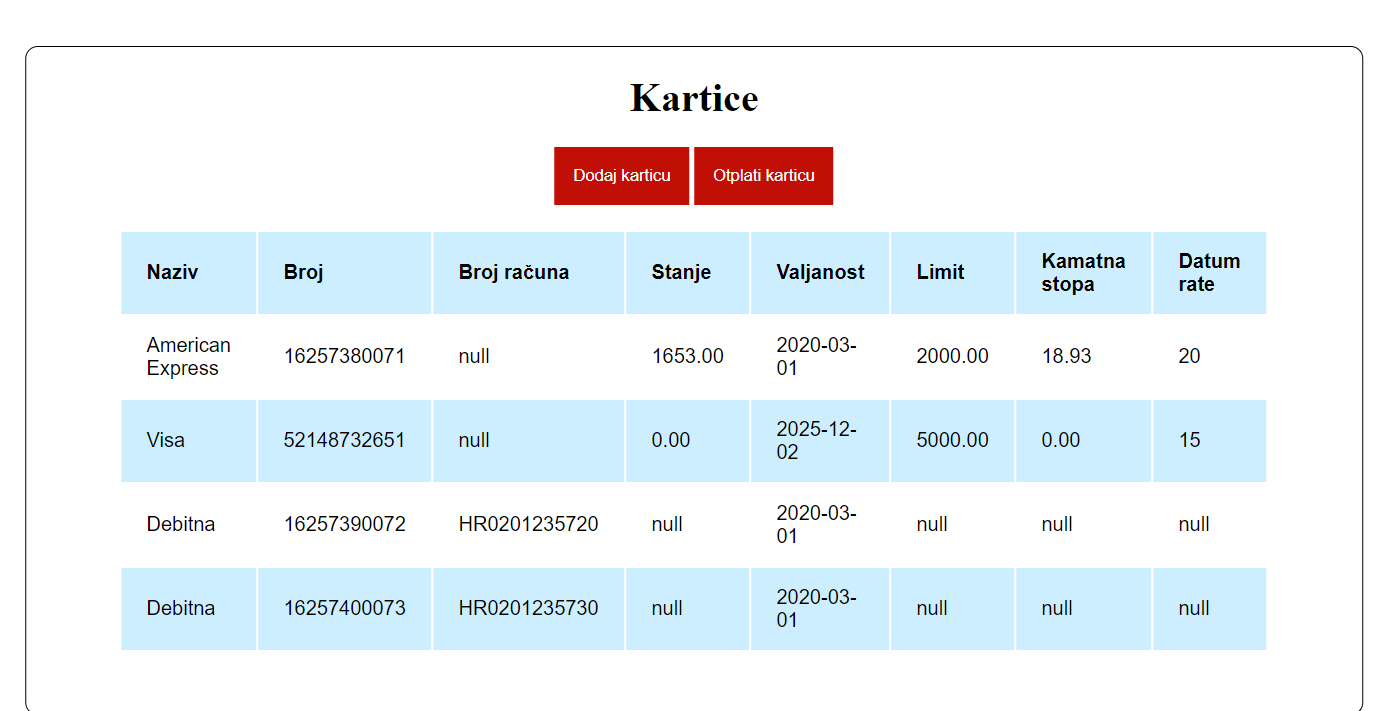
\includegraphics[scale=0.5]{slike/karticeposlije.PNG}
			\centering
			\caption{Prikaz kartica nakon odobravanja zahtjeva}
			\label{fig:poslije}
		\end{figure}
	
	\textbf{Ispitni slučaj 3: Provedba transakcije} 
	
	\textbf{Ulaz}
	
	\begin{enumerate}
		
		\item Otvaranje početne stranice u web pregledniku.
		\item Upisivanje korisničkog imena i lozinke klijenta.
		\item Odabir gumba "Nova transakcija".
		\item Odabir računa terećenja, računa odobrenja i iznos.
		
	\end{enumerate}
	
	\textbf{Očekivani rezultat}
	
	\begin{enumerate}
		\item Klijentu se u sustavu kod popisa transakcija ispisuje nova transakcija koju je proveo i detalji te transakcije.
		\item Klijent na čiji račun su poslani novci također kod transakcija vidi provedenu transakciju i detalje iste.
	\end{enumerate}
	
	\textbf{Rezultat}: Očekivani rezultat je zadovoljen i nakon prijave u sustav, klijent je uspješno obavio transakciju na drugi račun. Aplikacija je prošla test.
	
	\begin{figure}[H]
		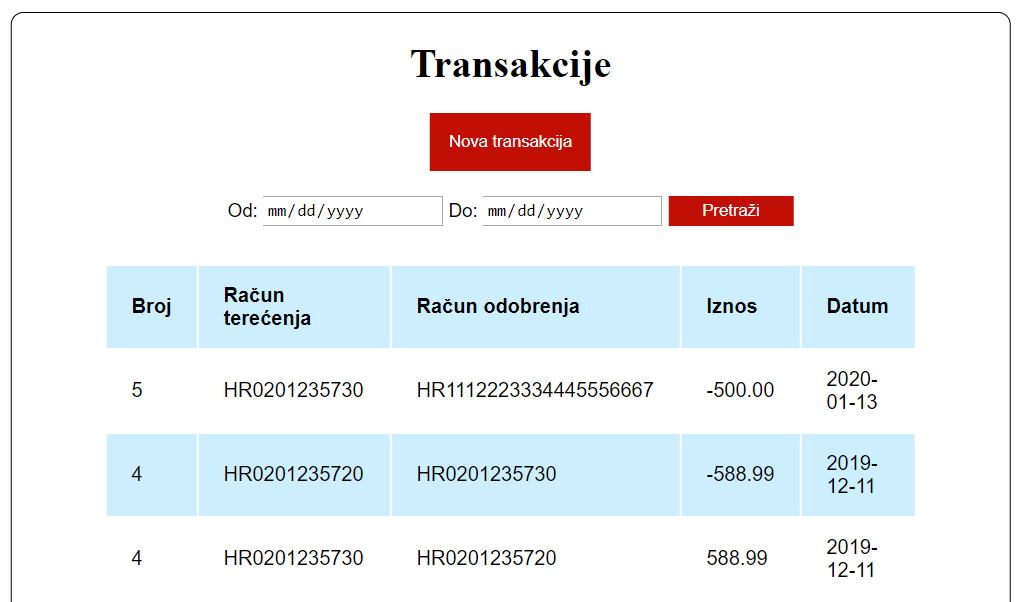
\includegraphics[scale=0.7]{slike/transakcijeprije.PNG}
		\centering
		\caption{Prikaz transakcija prije obavljanja transakcije}
		\label{fig:transprije}
	\end{figure}
	\begin{figure}[H]
		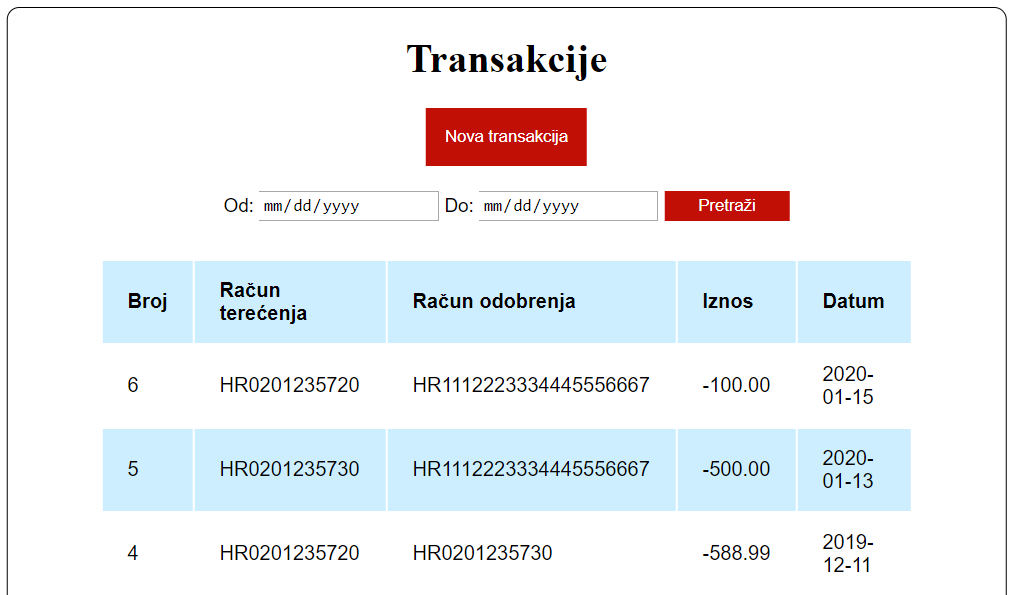
\includegraphics[scale=0.7]{slike/transakcijeposlije.PNG}
		\centering
		\caption{Prikaz detalja transakcije poslije navedene transakcije}
		\label{fig:transposlije}
	\end{figure}

	\textbf{Ispitni slučaj 4: Izrada novog računa} 
	
	\textbf{Ulaz}
	
	\begin{enumerate}
		
		\item Otvaranje početne stranice u web pregledniku.
		\item Upisivanje korisničkog imena i lozinke bankara.
		\item Odabir gumba "Dodaj račun".
		\item Popunjavanje obaveznih polja za stvaranje novog računa.
		
	\end{enumerate}
	
	\textbf{Očekivani rezultat}
	
	\begin{enumerate}
		\item Bankar nakon upisivanja OIB-a klijenta, koji je želio otvoriti novi račun, ima uvid u sve otvorene račune.
		\item Klijentu se prikazuju svi računi koje je otvorio.
	\end{enumerate}
	
	\textbf{Rezultat}: Očekivani rezultat je zadovoljen i bankar je uspješno otvorio račun određenom klijentu. Aplikacija je prošla test.
	
	\begin{figure}[H]
		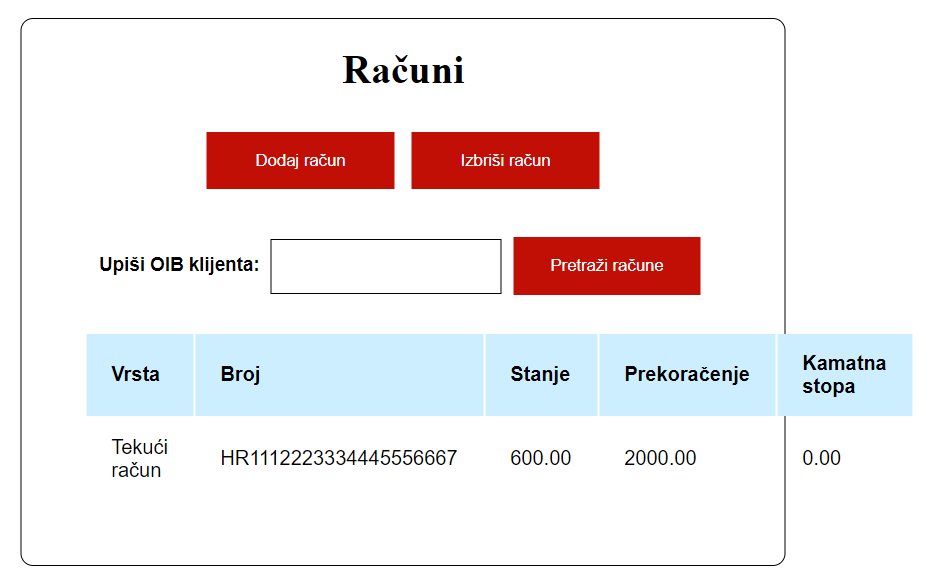
\includegraphics[scale=0.7]{slike/racuniklijentaprije.PNG}
		\centering
		\caption{Prikaz svih otvorenih računa prije zahtjeva za otvranjem novo računa}
		\label{fig:racprije}
	\end{figure}
	\begin{figure}[H]
		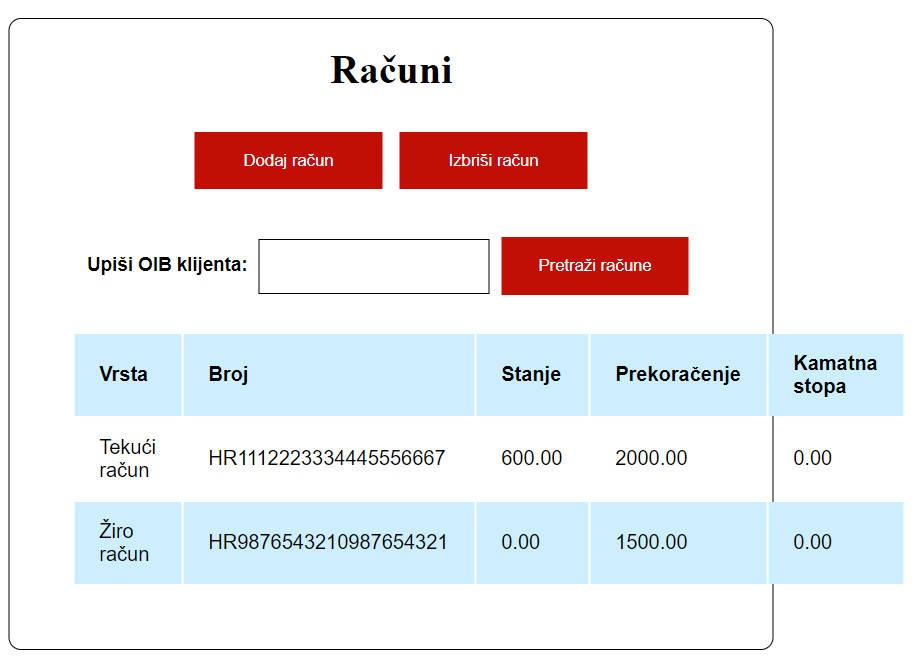
\includegraphics[scale=0.7]{slike/racuniklijentaposlije.PNG}
		\centering
		\caption{Prikaz svih otvorenih računa nekog klijenta poslije otvaranja novog računa}
		\label{fig:racposlije}
	\end{figure}

			
			\eject 
		
		
		\section{Dijagram razmještaja}
			
			\textbf{\textit{dio 2. revizije}}
			
			 \textit{Potrebno je umetnuti \textbf{specifikacijski} dijagram razmještaja i opisati ga. Moguće je umjesto specifikacijskog dijagrama razmještaja umetnuti dijagram razmještaja instanci, pod uvjetom da taj dijagram bolje opisuje neki važniji dio sustava.}
			
			
		
			\eject 
		
		\section{Upute za puštanje u pogon}
		
			\textbf{\textit{dio 2. revizije}}\\
		
			 \textit{U ovom poglavlju potrebno je dati upute za puštanje u pogon (engl. deployment) ostvarene aplikacije. Na primjer, za web aplikacije, opisati postupak kojim se od izvornog kôda dolazi do potpuno postavljene baze podataka i poslužitelja koji odgovara na upite korisnika. Za mobilnu aplikaciju, postupak kojim se aplikacija izgradi, te postavi na neku od trgovina. Za stolnu (engl. desktop) aplikaciju, postupak kojim se aplikacija instalira na računalo. Ukoliko mobilne i stolne aplikacije komuniciraju s poslužiteljem i/ili bazom podataka, opisati i postupak njihovog postavljanja. Pri izradi uputa preporučuje se \textbf{naglasiti korake instalacije uporabom natuknica} te koristiti što je više moguće \textbf{slike ekrana} (engl. screenshots) kako bi upute bile jasne i jednostavne za slijediti.}
			
			
			 \textit{Dovršenu aplikaciju potrebno je pokrenuti na javno dostupnom poslužitelju. Studentima se preporuča korištenje neke od sljedećih besplatnih usluga: \href{https://aws.amazon.com/}{Amazon AWS}, \href{https://azure.microsoft.com/en-us/}{Microsoft Azure} ili \href{https://www.heroku.com/}{Heroku}. Mobilne aplikacije trebaju biti objavljene na F-Droid, Google Play ili Amazon App trgovini.}
			
			
			\eject 